\section{T2K}

The T2K experiment uses an off-axis $\nu_\mu$ beam produced from $\pi^+ \to \mu^+ \nu_\mu$ decays. Consider the case where the pion has velocity $\beta$ along the $z$-direction in the laboratory frame and a neutrino with energy $E^*$ is produced at an angle $\theta^*$ with respect to the $z'$-axis in the $\pi^+$ rest frame.

\begin{enumerate}[label=\textbf{\alph*}.]
    \item Show that the neutrino energy in the pion rest frame is $p^* = (m_\pi^2 - m_\mu^2) / 2m_\pi$

    We know that for any decay of the form $a \to 1 + 2$, we have
    \begin{align*}
      p^* &= \frac{1}{2m_a}\sqrt{\left[m_a^2 - (m_1+m_2)^2\right]\left[m_a^2 - (m_1-m_2)^2\right]} \\
    \end{align*}

    In our case, $\pi^+ \to \mu^+ \nu_\mu$
    \begin{align*}
      p^* &= \frac{1}{2m_\pi}\sqrt{\left[m_\pi^2 - (m_\mu+m_\nu)^2\right]\left[m_\pi^2 - (m_\nu-m_\mu)^2\right]} \\
      &\approx \frac{1}{2m_\pi}\sqrt{\left[m_\pi^2 - (0+m_\nu)^2\right]\left[m_\pi^2 - (0-m_\mu)^2\right]} \\
      &= \frac{m_\pi^2 - m_\mu^2}{2m_\pi} \\
    \end{align*}

    \item Using a Lorentz transformation, show that the energy $E$ and angle of production $\theta$ of the neutrino in the lab frame are $E = \gamma E^*(1 + \beta \cos(\theta^*)), E\cos(\theta) = \gamma E^*(\cos(\theta^*) + \beta)$, where $\gamma = E_\pi/m_\pi$.

    In the rest frame, we have
    \begin{align*}
        p_\pi^* &= (m_\pi, 0, 0, 0) \\
        p_\nu^* &= p^*(1, \sin(\theta^*), 0, \cos(\theta^*)) \\
        p_\mu^* &= (m_\pi-p^*, -p^*\sin(\theta^*), 0, -p^*\cos(\theta^*)) \\
    \end{align*}

    And in the lab frame we'll have
    \begin{align*}
        p_\pi &= (E_\pi, 0, 0, m_\pi\beta) \\
        p_\nu &= p(1, \sin(\theta), 0, \cos(\theta)) \\
        p_\mu &= (E_\pi-p, -p\sin(\theta), 0, -p\cos(\theta)) \\
    \end{align*}

    First show $\gamma = \frac{E_\pi}{m_\pi}$ using the Lorentz transformations for momentum/energy (boost with $-\beta$ to get into the lab frame):
    \begin{align*}
        E_\pi &= \gamma(E_\pi^* + \beta p_{z,\pi}^*) \\
        E_\pi &= \gamma((m_\pi) + \beta (0)) \\
        E_\pi &= \gamma m_\pi \\
        \gamma &= \frac{E_\pi}{m_\pi}\\
    \end{align*}

    Then on use the same transformations on the neutrino, and also use $p^* = E^*$ for the neutrino since it's essentially massless:
    \begin{align*}
        E &= \gamma(E^* + \beta p_{z,\nu}^*) \\
        &= \gamma(E^* + \beta p^*\cos(\theta^*)) \\
        &= \gamma(E^* + \beta E^*\cos(\theta^*)) \\
        &= \gamma E^*(1 + \beta \cos(\theta^*)) \\
        p_{z,\nu} &= \gamma(p_{z,\nu}^* + \beta E^*) \\
        E\cos(\theta) &= \gamma(p^*\cos(\theta^*) + \beta E^*) \\
        &= \gamma(E^*\cos(\theta^*) + \beta E^*) \\
        &= \gamma E^*(\cos(\theta^*) + \beta) \\
    \end{align*}
    
    \item Using the expressions for $E^*$ and $\theta^*$ in terms of $E$ and $\theta$, show that $\gamma^2 (1 - \beta\cos(\theta))(1 + \beta\cos(\theta^*)) = 1$

    Derive a similar expression to the ones above for the unstarred $E, \theta$, flipping the sign on $\beta$ for the inverse transform:

    \begin{align*}
        E^* &= \gamma(E - \beta p_{z,\nu}) \\
        &= \gamma(E - \beta p\cos(\theta)) \\
        &= \gamma(E - \beta E\cos(\theta)) \\
        &= \gamma E(1 - \beta \cos(\theta)) \\
    \end{align*}

    Use this:
    \begin{align*}
        \gamma^2 (1 - \beta\cos(\theta))(1 + \beta\cos(\theta^*)) &= \frac{1}{E}\gamma E(1 - \beta\cos(\theta)) \frac{1}{E^*}\gamma E^*(1 + \beta \cos(\theta^*))\\
        &= \frac{1}{E}E^* \frac{1}{E^*}E\\
        &= \frac{EE^*}{EE^*}\\
        &= 1\\
    \end{align*}

    \item Assuming that the pions have a flat energy spectrum in the range $1-\SI{5}{GeV}$, sketch the form of the resulting neutrino energy spectrum at the T2K far detector (SuperK), which is off-axis at $\theta=2.5^\circ$. Given that SuperK is 295km from the beam, explain why this angle was chosen.

    First, get an expression for $\beta$:
    \begin{align*}
        \gamma &= \frac{1}{\sqrt{1 - \beta^2}}
        \implies \beta = \sqrt{1 - \frac{1}{\gamma^2}}
    \end{align*}

    And use our other knowledge from above to get an expression for $E_\nu$ in terms of other variables we have:
    \begin{align*}
        E_\nu^* &= \gamma E_\nu(1 - \beta \cos(\theta)) \\
        p^* &= \gamma E_\nu(1 - \beta \cos(\theta)) \\
        \frac{m_\pi^2 - m_\mu^2}{2m_\pi} &= \frac{E_\pi}{m_\pi} E_\nu(1 - \beta \cos(\theta)) \\
        \frac{m_\pi^2 - m_\mu^2}{2E_\pi(1 - \beta \cos(\theta))} &= E_\nu \\
        \frac{m_\pi^2 - m_\mu^2}{2E_\pi\left(1 - \sqrt{1 - \frac{m_\pi^2}{E_\pi^2}} \cos(\theta)\right)} &= E_\nu \\
    \end{align*}

    \newpage
    This is something we can plot for different values of $\theta$:
    \begin{center}
        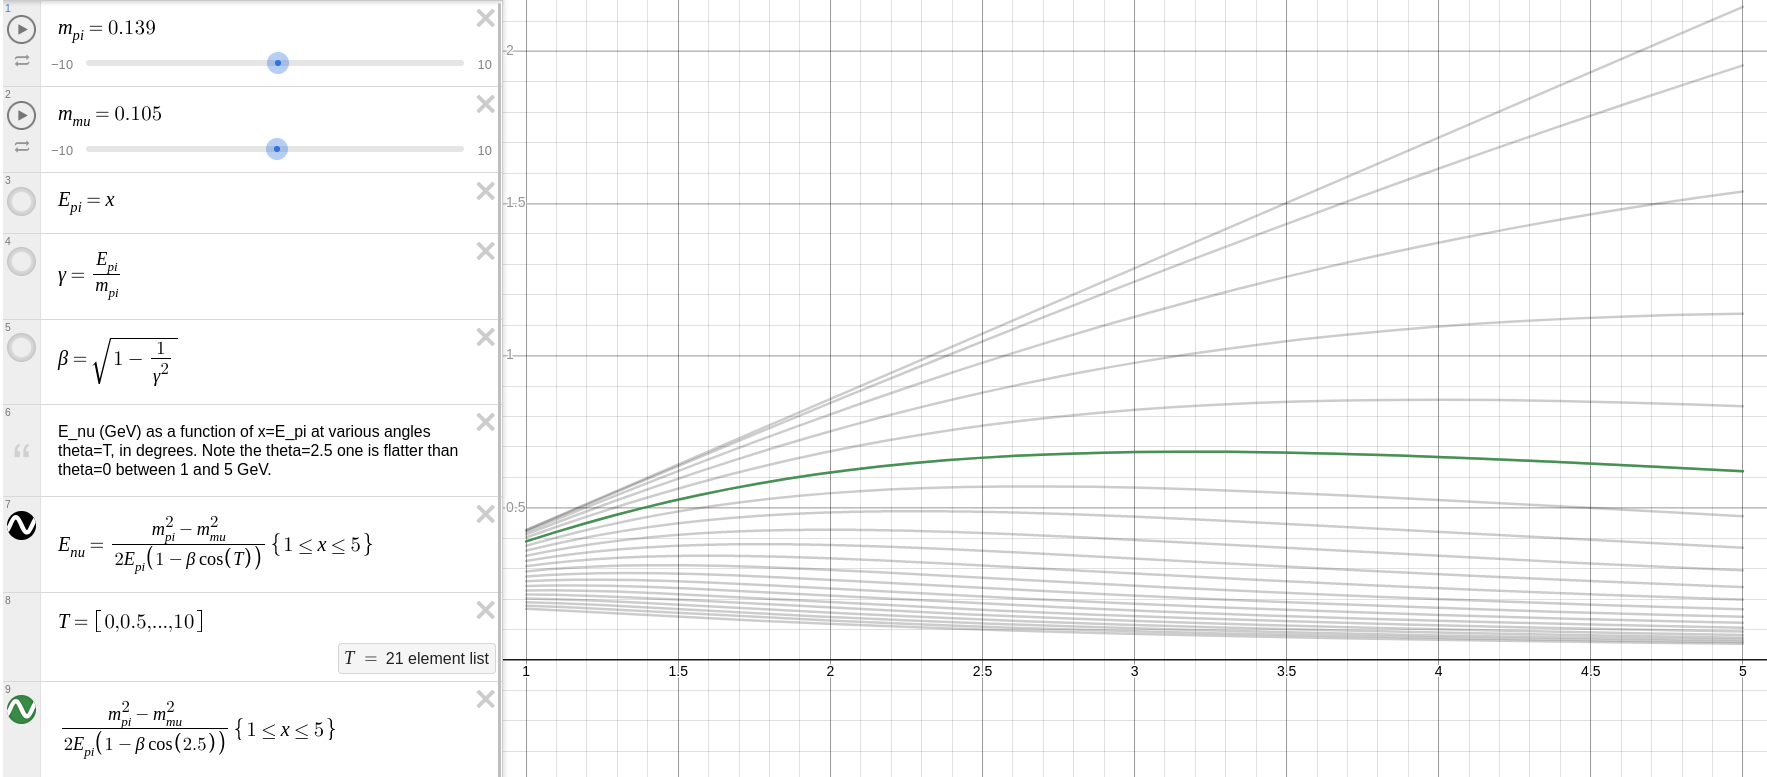
\includegraphics[width=0.9\textwidth]{q5.png}

        \small{$E_\nu$ (GeV) as a function of $E_\pi$ at various angles $\theta$, in degrees.
        
        Note the $\theta=2.5$ line is flatter than $\theta=0$ between 1 and 5 GeV.}
    \end{center}

    I suppose at a large distance like 295km, it's a good idea to have a more energy-uniform beam of neutrinos, so you can tell which ones came from the experiment vs external sources and also so you only need to design detectors to measure within a smaller range of energies, hence the choice of 2.5$^\circ$.

  \end{enumerate}

